\documentclass{article}

\usepackage{tikz}
\usetikzlibrary{shapes.multipart,positioning}

\usepackage{listings}

\begin{document}
  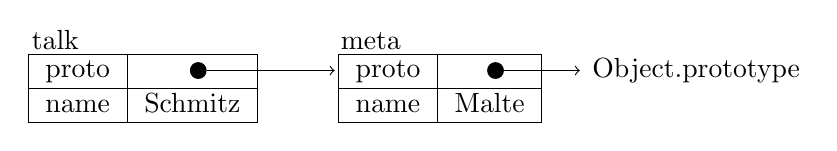
\begin{tikzpicture}[shorten >=1pt]
    \node[inner sep=0pt] (talk) {
      \begin{tabular}{|l|l|}
        \hline
        proto & \\ \hline
        \lstinline-name- & \lstinline-Schmitz- \\ \hline 
      \end{tabular}
    };
    \node[anchor=south west,inner sep=1pt] at (talk.north west) {\lstinline-talk-};
    \node[circle,draw,fill,inner sep=2pt,xshift=2em,yshift=1.5ex] at (talk.center) (talk dot) {};
    \node[inner sep=0pt,right=of talk] (meta) {
      \begin{tabular}{|l|l|}
        \hline
        proto & \\ \hline
        \lstinline-name- & \lstinline-Malte- \\ \hline 
      \end{tabular}
    };
    \node[anchor=south west,inner sep=1pt] at (meta.north west) {\lstinline-meta-};
    \node[circle,draw,fill,inner sep=2pt,xshift=2em,yshift=1.5ex] at (meta.center) (meta dot) {};
    \node[right=of meta dot] (obj) {\lstinline-Object.prototype-};
    \draw[->] (talk dot) edge (meta.west |- talk dot);
    \draw[->] (meta dot) edge (obj);
  \end{tikzpicture}
\end{document}